\documentclass{wissdoc}
% Autor: Roland Bless 1996-2009, bless <at> kit.edu
% ----------------------------------------------------------------
% Diplomarbeit - Hauptdokument
% ----------------------------------------------------------------
%%
%% $Id: thesis.tex 65 2012-05-10 10:32:11Z bless $
%%
% wissdoc Optionen: draft, relaxed, pdf --> siehe wissdoc.cls
% ------------------------------------------------------------------
% Weitere packages: (Dokumentation dazu durch "latex <package>.dtx")
\usepackage[numbers,sort&compress]{natbib}
% \usepackage{varioref}
% \usepackage{verbatim}
% \usepackage{float}    %z.B. \floatstyle{ruled}\restylefloat{figure}
% \usepackage{subfigure}
% \usepackage{fancybox} % f�r schattierte,ovale Boxen etc.
% \usepackage{tabularx} % automatische Spaltenbreite
% \usepackage{supertab} % mehrseitige Tabellen
% \usepackage[svnon,svnfoot]{svnver} % SVN Versionsinformation 
%% ---------------- end of usepackages -------------

%\svnversion{$Id: thesis.tex 65 2012-05-10 10:32:11Z bless $} % In case that you want to include version information in the footer

%% Informationen f�r die PDF-Datei
\hypersetup{
 pdfauthor={N.N.},
 pdftitle={Not set}
 pdfsubject={Not set},
 pdfkeywords={Not set}
}

% Macros, nicht unbedingt notwendig
%%%%%%%%%%%%%%%%%%%%%%%%%%%%%%%%%%%%%%%%%%%%%%%%%%%%%%%%%%
% macros.tex -- einige mehr oder weniger nuetzliche Makros
% Autor: Roland Bless 1998
%%%%%%%%%%%%%%%%%%%%%%%%%%%%%%%%%%%%%%%%%%%%%%%%%%%%%%%%%%
% $Id: macros.tex 33 2007-01-23 09:00:59Z bless $
%%%%%%%%%%%%%%%%%%%%%%%%%%%%%%%%%%%%%%%%%%%%%%%%%%%%%%%%%%


%%%%%%%%%%%%%%%%%%%%%%%
% Kommentare 
%%%%%%%%%%%%%%%%%%%%%%%
\ifnotdraftelse{
\newcommand{\Kommentar}[1]{}
}{\newcommand{\Kommentar}[1]{{\em #1}}}
% Alles innerhalb von \Hide{} oder \ignore{} 
% wird von LaTeX komplett ignoriert (wie ein Kommentar)
\newcommand{\Hide}[1]{}
\let\ignore\Hide

%%%%%%%%%%%%%%%%%%%%%%%%%
% Leere Seite ohne Seitennummer, wird aber gezaehlt
%%%%%%%%%%%%%%%%%%%%%%%%%

\newcommand{\leereseite}{% Leerseite ohne Seitennummer, nächste Seite rechts (wenn 2-seitig)
 \clearpage{\pagestyle{empty}\cleardoublepage}
}
%%%%%%%%%%%%%%%%%%%%%%%%%%
% Flattersatz rechts und Silbentrennung, Leerraum nach rechts maximal 1cm
%%%%%%%%%%%%%%%%%%%%%%%%%%
\makeatletter
\newcommand{\myraggedright}{%
 \let\\\@centercr\@rightskip 0pt plus 1cm
 \rightskip\@rightskip
  \leftskip\z@skip
  \parindent\z@
  \spaceskip=.3333em
  \xspaceskip=.5em}
\makeatother

\makeatletter
\newcommand{\mynewline}{%
 \@centercr\@rightskip 0pt plus 1cm
}
\makeatother


%%%%%%%%%%%%%%%%%%%%%%%%%%
% Für Index
%%%%%%%%%%%%%%%%%%%%%%%%%%
\makeatletter
\def\mydotfill{\leavevmode\xleaders\hb@xt@ .44em{\hss.\hss}\hfill\kern\z@}
\makeatother
\def\bold#1{{\bfseries #1}}
\newbox\dbox \setbox\dbox=\hbox to .4em{\hss.\hss} % dot box for leaders
\newskip\rrskipb \rrskipb=.5em plus3em % ragged right space before break
\newskip\rrskipa \rrskipa=-.17em plus -3em minus.11em % ditto, after
\newskip\rlskipa \rlskipa=0pt plus3em % ragged left space after break
\newskip\rlskipb \rlskipb=.33em plus-3em minus.11em % ragged left before break
\newskip\lskip \lskip=3.3\wd\dbox plus1fil minus.3\wd\dbox % for leaders
\newskip \lskipa \lskipa=-2.67em plus -3em minus.11em %after leaders
\mathchardef\rlpen=1000 \mathchardef\leadpen=600
\def\rrspace{\nobreak\hskip\rrskipb\penalty0\hskip\rrskipa}
\def\rlspace{\penalty\rlpen\hskip\rlskipb\vadjust{}\nobreak\hskip\rlskipa}
\let\indexbreak\rlspace
\def\raggedurl{\penalty10000 \hskip.5em plus15em \penalty0 \hskip-.17em plus-15em minus.11em}
\def\raggeditems{\nobreak\hskip\rrskipb \penalty\leadpen \hskip\rrskipa %
\vadjust{}\nobreak\leaders\copy\dbox\hskip\lskip %
\kern3em \penalty\leadpen \hskip\lskipa %
\vadjust{}\nobreak\hskip\rlskipa}
\renewcommand*\see[2]{\rlspace\emph{\seename}~#1} % from makeidx.sty

%%%%%%%%%%%%%%%%%%%%%%%%%%
% Neue Seite rechts, leere linke Seite ohne Headings
%%%%%%%%%%%%%%%%%%%%%%%%%%
\newcommand{\xcleardoublepage}
{{\pagestyle{empty}\cleardoublepage}}

%%%%%%%%%%%%%%%%%%%%%%%%%%
% Tabellenspaltentypen (benoetigt colortbl)
%%%%%%%%%%%%%%%%%%%%%%%%%%
\newcommand{\PBS}[1]{\let\temp=\\#1\let\\=\temp}
\newcolumntype{y}{>{\PBS{\raggedright\hspace{0pt}}}p{1.35cm}}
\newcolumntype{z}{>{\PBS{\raggedright\hspace{0pt}}}p{2.5cm}}
\newcolumntype{q}{>{\PBS{\raggedright\hspace{0pt}}}p{6.5cm}}
\newcolumntype{g}{>{\columncolor[gray]{0.8}}c} % Grau
\newcolumntype{G}{>{\columncolor[gray]{0.9}}c} % helleres Grau

%%%%%%%%%%%%%%%%%%%%%%%%%%
% Anführungszeichen oben und unten
%%%%%%%%%%%%%%%%%%%%%%%%%%
\newcommand{\anf}[1]{"`{#1}"'}

%%%%%%%%%%%%%%%%%%%%%%%%%%
% Tiefstellen von Text
%%%%%%%%%%%%%%%%%%%%%%%%%%
% S\tl{0} setzt die 0 unter das S (ohne Mathemodus!)
% zum Hochstellen gibt es uebrigens \textsuperscript
\makeatletter
\DeclareRobustCommand*\textlowerscript[1]{%
  \@textlowerscript{\selectfont#1}}
\def\@textlowerscript#1{%
  {\m@th\ensuremath{_{\mbox{\fontsize\sf@size\z@#1}}}}}
\let\tl\textlowerscript
\let\ts\textsuperscript
\makeatother

%%%%%%%%%%%%%%%%%%%%%%%%%%
% Gauß-Klammern
%%%%%%%%%%%%%%%%%%%%%%%%%%
\newcommand{\ceil}[1]{\lceil{#1}\rceil}
\newcommand{\floor}[1]{\lfloor{#1}\rfloor}

%%%%%%%%%%%%%%%%%%%%%%%%%%
% Average Operator (analog zu min, max)
%%%%%%%%%%%%%%%%%%%%%%%%%%
\def\avg{\mathop{\mathgroup\symoperators avg}}

%%%%%%%%%%%%%%%%%%%%%%%%%%
% Wortabkürzungen
%%%%%%%%%%%%%%%%%%%%%%%%%%
\def\zB{z.\,B.\ }
\def\dh{d.\,h.\ }
\def\ua{u.\,a.\ }
\def\su{s.\,u.\ }
\newcommand{\bzw}{bzw.\ }

%%%%%%%%%%%%%%%%%%%%%%%%%%%%%%%%%%%
% Einbinden von Graphiken
%%%%%%%%%%%%%%%%%%%%%%%%%%%%%%%%%%%
% global scaling factor
\def\gsf{0.9}
%% Graphik, 
%% 3 Argumente: Datei, Label, Unterschrift
\newcommand{\Abbildung}[3]{%
\begin{figure}[tbh] %
\centerline{\scalebox{\gsf}{\includegraphics*{#1}}} %
\caption{#3} %
\label{#2} %
\end{figure} %
}
\let\Abb\Abbildung
%% Abbps
%% Graphik, skaliert, Angabe der Position
%% 5 Argumente: Position, Breite (0 bis 1.0), Datei, Label, Unterschrift
\newcommand{\Abbildungps}[5]{%
\begin{figure}[#1]%
\begin{center}
\scalebox{\gsf}{\includegraphics*[width=#2\textwidth]{#3}}%
\caption{#5}%
\label{#4}%
\end{center}
\end{figure}%
}
\let\Abbps\Abbildungps
%% Graphik, Angabe der Position, frei wählbares Argument für includegraphics
%% 5 Argumente: Position, Optionen, Datei, Label, Unterschrift
\newcommand{\Abbildungpf}[5]{%
\begin{figure}[#1]%
\begin{center}
\scalebox{\gsf}{\includegraphics*[#2]{#3}}%
\caption{#5}%
\label{#4}%
\end{center}
\end{figure}%
}
\let\Abbpf\Abbildungpf

%%
% Anmerkung: \resizebox{x}{y}{box} skaliert die box auf Breite x und Höhe y,
%            ist x oder y ein !, dann wird das usprüngliche 
%            Seitenverhältnis beibehalten.
%            \rescalebox funktioniert ähnlich, nur das dort ein Faktor
%            statt einer Dimension angegeben wird.
%%
% \Abbps{Position}{Breite in Bruchteilen der Textbreite}{Dateiname}{Label}{Bildunterschrift}
%

\newcommand{\refAbb}[1]{%
s.~Abbildung \ref{#1}}

%%%%%%%%%%%%%%%%%%%%
%% end of macros.tex
%%%%%%%%%%%%%%%%%%%%

% Print URLs not in Typewriter Font
\def\UrlFont{\rm}

\newcommand{\blankpage}{% Leerseite ohne Seitennummer, n�chste Seite rechts
 \clearpage{\pagestyle{empty}\cleardoublepage}
}

%% Einstellungen f�r das gesamte Dokument

% Trennhilfen
% Wichtig! 
% Im ngerman-paket sind zus�tzlich folgende Trennhinweise enthalten:
% "- = zus�tzliche Trennstelle
% "| = Vermeidung von Ligaturen und m�gliche Trennung (bsp: Schaf"|fell)
% "~ = Bindestrich an dem keine Trennung erlaubt ist (bsp: bergauf und "~ab)
% "= = Bindestrich bei dem Worte vor und dahinter getrennt werden d�rfen
% "" = Trennstelle ohne Erzeugung eines Trennstrichs (bsp: und/""oder)

% Trennhinweise fuer Woerter hier beschreiben
\hyphenation{
% Pro-to-koll-in-stan-zen
% Ma-na-ge-ment  Netz-werk-ele-men-ten
% Netz-werk Netz-werk-re-ser-vie-rung
% Netz-werk-adap-ter Fein-ju-stier-ung
% Da-ten-strom-spe-zi-fi-ka-tion Pa-ket-rumpf
% Kon-troll-in-stanz
}

% Index-Datei �ffnen
\ifnotdraft{\makeindex}
%%%%%%%%%%%%%% includeonly %%%%%%%%%%%%%%%%%%%
% Es werden nur die Teile eingebunden, die hier 
% aufgefuehrt sind!
\includeonly{%
titelseite,%
erklaerung,% Ist in KA Pflicht f�r Diplomarbeiten
einleitung,% Motivation, Zielsetzung, Gliederung
grundlagen,% Grundlagen 
analyse,   % Problembeschreibung (Detail) und Related Work
entwurf,   % Beschreibung der Probleml�sung (Konzepte, allg. Architektur, ...)
implemen,  % Beschreibung der Umsetzung/Implementierung
eval,      % Nachweis und Auswertung
zusammenf  % Zusammenfassung der Ergebnisse und Ausblick
}
%%%%%%%%%%%%%%%%%%%%%%%%%%%%%%%%%%%%%%%%%%%%%%
\begin{document}

\frontmatter
\pagenumbering{roman}
\ifnotdraft{
 %% Titelseite
%% Vorlage $Id: titelseite.tex 61 2012-05-03 13:58:03Z bless $

\def\usesf{}
\let\usesf\sffamily % diese Zeile auskommentieren für normalen TeX Font

\newsavebox{\Erstgutachter}
\savebox{\Erstgutachter}{\usesf Prof.~Dr.~?.~?????????}
\newsavebox{\Zweitgutachter}
\savebox{\Zweitgutachter}{\usesf Prof.~Dr.~?.~?????????}

\begin{titlepage}
\setlength{\unitlength}{1pt}
\begin{picture}(0,0)(85,770)

\includegraphics[width=\paperwidth]{logos/HFTL_Deckblatt}
\end{picture}

\thispagestyle{empty}

%\begin{titlepage}
%%\let\footnotesize\small \let\footnoterule\relax
\begin{center}
\hbox{}
\vfill
{\usesf
{\huge\bfseries Quantified Self\\
                Diplom-/Studien-/Master-/""Bachelorarbeit \par}
\vskip 1.8cm
Diplomarbeit/Studienarbeit/Masterarbeit/Bachelorarbeit\\
von\\[2mm]
\vskip 1cm

{\large\bfseries Chi Trung Nguyen\\
Florian Weber}
\vskip 1.2cm
am Institut für Telematik\\
der Fakultät für Informatik\\
%Universität Karlsruhe (TH)\\[2ex]
\vskip 3cm
\begin{tabular}{p{5.5cm}l}
Erstgutachter: & \usebox{\Erstgutachter} \\
Zweitgutachter: & \usebox{\Zweitgutachter} \\
Betreuender~Mitarbeiter: & Dipl.-Inform.~?.~????????? \\
\end{tabular}
\vskip 3cm
Bearbeitungszeit:\qquad ??.~Monat~20?? -- ??.~Monat~20??
}
\end{center}
\vfill
\end{titlepage}
%% Titelseite Ende


%%% Local Variables: 
%%% mode: latex
%%% TeX-master: "thesis"
%%% End: 

 \blankpage % Leerseite auf Titelr�ckseite
 %
 % Die folgende Erkl�rung ist f�r Diplomarbeiten Pflicht
 % (siehe Pr�fungsordnung), f�r Studienarbeiten nicht notwendig
 \thispagestyle{empty}
\vspace*{42\baselineskip}
\hbox to \textwidth{\hrulefill}
\par
Ich erkläre hiermit, dass ich die vorliegende Arbeit selbständig verfasst und
keine anderen als die angegebenen Quellen und Hilfsmittel verwendet habe.

Leipzig, den ??. ?????? 201?

%%%%%%%%%%%%%%%%%%%%%%%%%%%%%%%%%%%%%%%%%%%%%%%%%%%%%%%%%%%%%%%%%%%%%%%%
%% Hinweis:
%%
%% Diese Erklärung wird von der Prüfungsordnung für Diplomarbeiten 
%% verlangt und ist zu unterschreiben. Für Studienarbeiten ist diese
%% Erklärung nicht zwingend notwendig, schadet aber auch nicht.
%%%%%%%%%%%%%%%%%%%%%%%%%%%%%%%%%%%%%%%%%%%%%%%%%%%%%%%%%%%%%%%%%%%%%%%%
\clearpage







 \blankpage % Leerseite auf Erkl�rungsr�ckseite
}
%
%% *************** Hier geht's ab ****************
%% ++++++++++++++++++++++++++++++++++++++++++
%% Verzeichnisse
%% ++++++++++++++++++++++++++++++++++++++++++
\ifnotdraft{
{\parskip 0pt\tableofcontents} % toc bitte einzeilig
\blankpage
%\listoffigures
%\blankpage
%\listoftables
%\blankpage
}


%% ++++++++++++++++++++++++++++++++++++++++++
%% Hauptteil
%% ++++++++++++++++++++++++++++++++++++++++++
\graphicspath{{Bilder/}}

\mainmatter
\pagenumbering{arabic}
%% Einleitung.tex
%% $Id: einleitung.tex 61 2012-05-03 13:58:03Z bless $
%%

\chapter{Einleitung}
\label{ch:Einleitung}
%% ==============================

%% ==============================
\section{Problemstellung}
%% ==============================
\label{ch:Einleitung:sec:Problemstellung}

Seit Gründung der Initiative \href{http://quantifiedself.com/}{\textbf{Quantified Self}}(QS) im \href{http://quantifiedself.com/2011/03/what-is-the-quantified-self/}{\textbf{Jahr 2007}} steigen die Möglichkeiten von Jahr zu Jahr, Umwelt und personenbezogene Daten zu erfassen. \cite{web:Tracking} 
Dies wird durch unterschiedliche Hard und Softwarelösungen ermöglicht. \\
Dabei werden Erkenntnisse über Gesundheit, Fitness und persönliche Stimmung gesammelt.
Diese können auch zu externen Umweltfaktoren in Relation gebracht werden. \\
Als Leitfrage des Projekts wurde die Frage, ob durch Quantified Self das Leben verbessert werden kann, festgesetzt. 
Das Erreichen des Ziels, die Beantwortung der Leitfrage durch das Analysieren und Auswerten von aus Selbstversuchen gewonnener Daten[...].
Zur Zielerreichung wird zu Beginn der Datengenerierungs- bzw. Testphase, die 30 Tage beträgt, der augenblickliche Zustand der Probanden aufgezeichnet und gesichert –– also der derzeitige Schlafrhythmus, die derzeitige Essgewohnheit und die Bewegungsaktivität.
Dieser wird als 100\% Marke angesetzt und dient der späteren Auswertung der gewonnen Daten als Maßstab. 
Die Daten werden aus Bewegungsaktivität, Schlafrhythmus und Stimmungslage gewonnen 
Sollte der analysierte Wert nach der Testphase über dieser Marke liegen, liegt eindeutig eine Verbesserung vor. 
Ist der Wert darunter, so stellt dieser eine Verschlechterung dar. \\
Zur besseren Klassifizierung der Daten wird von einer Verbesserung erst ab dem Wert von mindestens 120\% gesprochen, sowie von einer Verschlechterung bei einem Wert von 80\%. Sollte der Endwert eines Probanden zwischen 80\% und 120\% liegen wird von einem Gleichbleiben des Befindens gesprochen.
In der heutigen Zeit, in der die Lebenssituation, vor allem in der arbeitenden Bevölkerung, an Qualität abnimmt – sei es durch Stress im Arbeitsalltag oder der gewaltigen Informationsflut, die uns unterbewusst immer und überall beeinträchtigt – ist es wichtig, neue Möglichkeiten auszuloten, um die Lebensqualität zum Beispiel durch die Selbstanalyse diverser Faktoren wieder zu verbessern. 

\section{Zielsetzung}
%% ==============================
\label{ch:Einleitung:sec:Zielsetzung}

In diesem Projekt werden Faktoren wie Schlaf, Ernährung und Bewegungsaktivität sein, die mit Hilfe von Quantified Self Appliaktionen für das Smartphone aufgezeichnet und später analysiert werden. %formulierung
Dadurch soll herausgefunden werden, ob eine Verbesserung durch die Nutzung von QS-Applikationen möglich ist. \\
Die stetig steigende Anzahl von Burnout-Patienten und die Selbsteinschätzung vieler Menschen in Deutschland, die entgegen dem eigentlichen Trend, eine sinkende Lebensqualität bemängeln, versuchen wir mit unserem Projekt eine Perspektive zu geben, wie man eventuell die Situation durch den Einsatz mobiler QS-Applikation für diverse Faktoren verbessern kann. 
Dieses Projekt soll eventuelle neue Möglichkeiten zur Verbesserung des Lebens durch das Nutzen von QS aufzeigen und helfen den Burnout zu verhindern bzw. Stress abzubauen und so das Gesundheitssystem teilweise entlasten, sowie das Lebensgefühl verbessern. 

%% ==============================
\section{Gliederung der Arbeit}
%% ==============================
\label{ch:Einleitung:sec:GliederungDerArbeit}

Die Arbeit ist in sieben Teile gegliedert:

\begin{enumerate}
\def\labelenumi{\arabic{enumi}.}
\itemsep1pt\parskip0pt\parsep0pt
\item
  Einleitung (Motivation, Trend)
\item
  Informationen zu Quantified Self (Studien, Trend, Medizinische
  Untersuchung)
\item
  Softwarebeschreibung (Erläuterung, Einführung)

  \begin{enumerate}
  \def\labelenumii{\alph{enumii}.}
  \itemsep1pt\parskip0pt\parsep0pt
  \item
    Moves (Bewegungsaktivität)\\
  \item
    Hueman (persönliches Wohlbefinden)\\
  \item
    SleepCycle (Schlafzyklen-Analyse)
  \end{enumerate}
\item
  Relativierung: Mögliche Fehlerquellen (technische, persönliche,
  falsche Wahrnehmung der eigenen Verfassung)
\item
  Auswertung der generierten App-Daten
\item
  Analyse der ausgewerteten Daten
\item
  Fazit (Beantwortung der Leitfrage)
\end{enumerate}

Die Einleitung soll einen Einblick in die Problemstellung und Zielsetzung der Arbeit, Motivation und Trend, sowie den Aufbau der Arbeit beschreiben.
Informationen zu Quantified Self gibt Aufschluss über aktuelle Studien zu Quantified Self sowie den Trend und Medizinische Untersuchungen.
Innerhalb die Softwarebeschreibung wird detaillierter auf die Auswahl der Apps eingegangen. \\
Zusätzlich sind deren Funktionsweise und Features hier beschrieben.
Die Relativierung beschreibt mögliche technische und persönliche Fehlerquellen bei der Anwendung, sowie die Problematik bei falscher Wahrnehmung der eigenen Verfassung.


Auswertung der generierten App-Daten


Analyse der ausgewerteten Daten


Das Fazit beantwortet die Leitfrage des Projektes und soll Aufschluss über mögliche Verbesserungsideen geben.

%% ==============================
\section{Auswahl der Trackingmethoden}
%% ==============================
\label{ch:Einleitung:sec:AuswahlDerTrackingmethoden}

Aufgrund der gegeben Mittel und dem Ziel die Fragestellung realitätsnah zu beantworten, beschränken wir unsere Tracking-Methoden auf reine Softwarelösungen. 
Diese können mit etlichen handelsüblichen Smartphones benutzt werden und liefern für weniger als 2\euro{} gute Ergebnisse. \cite{web:TrackingResults} \cite{web:AppPreis} \\
Die Arbeit orientiert sich an alltagsüblichen Situtationen. 
Daher benutzt das Projektteam einen Schrittzähler („Moves”), Schlafzykluserfassung („Sleep Cycle”) und einen Stimmungsbarometer („Hueman”).
Die Software wird im folgenden näher erläutert. \\
Die Zielgruppe, für die dieses Projekt ins Leben gerufen wurde, sind vor allem Smartphone-Nutzer, deren derzeitiges Leben, sei es durch Stress im Arbeitsalltag oder Burnout-ähnlichen Symptomen, verbesserungswürdig ist bzw. die die derzeitige Lebenssituation zu verbessern suchen(oder es auch einfach nur analysieren möchten).  

%%% Local Variables: 
%%% mode: latex
%%% TeX-master: "thesis"
%%% End: 
  % Einleitung
%% grundlagen.tex
%% $Id: grundlagen.tex 61 2012-05-03 13:58:03Z bless $
%%

\chapter{Grundlagen}
\label{ch:Grundlagen}
%% ==============================
Die Grundlagen müssen soweit beschrieben werden, dass ein Leser das Problem und die Problemlösung versteht.
Um nicht zuviel zu beschreiben, kann man das auch erst gegen Ende der Arbeit schreiben.


%% ==============================
\section{Quantified Self}
%% ==============================
\label{ch:Grundlagen:sec:QuantifiedSelf}

\subsection{Allgemein}
%% ==============================
\label{ch:Grundlagen:sec:QuantifiedSelf:subsec:Allgemein}

Quantified Self ist ein Ausdruck dafür, Technologien oder Anwendungen zu nutzen, um das tägliche Leben durch ständige Datenerfassung zu visualisieren.
Hauptsächliche Bereiche, die durch Quantified Self erfasst werden sollen sind z.B. Essgewohnheit (welche Lebensmittel verzehrt wurden), persönliches Wohlbefinden (Stimmung, Erregung, Sauerstoffgehalt im Blut) und die Leistung (mentale und physische). 
Umgangssprachlich wird eine solche Selbstüberwachung und -erkennung, die tragbare Sensoren (EEG, ECG-, Video-, etc.) und mobile Plattformen (tragbare Fittness-Gadgets, Smartphones/Tablets, etc.) verbindet, auch „self-tracking“ genannt. 
Durch den heutigen Stand der Technik ist es so jedem möglich, bisher unbekannte eigene biometrische Daten kostengünstig und bequem zu ermitteln.

\subsection{Einsatzgebiete}
%% ==============================
\label{ch:Grundlagen:sec:QuantifiedSelf:subsec:Einsatzgebiete}

Der Hauptanwendungsbereich von Quantified Self ist die Verbesserung der eigenen Gesundheit und des persönlichen Wohlbefindens. 
Für diesen Bereich gibt es viele Geräte und Applikationen, die die körperliche Aktivität, die Kalorienzufuhr, die Schlafqualität, die Körperhaltung und andere Faktoren des persönlichen Wohlbefindens analysieren und helfen, die gewonnenen Daten visuell verständlich darzulegen. 
Diese Gesundheitsüberwachung soll das persönliche Wohlbefinden des Nutzers aufrecht erhalten und so potentielle Krankheiten verhindern.
Die daraus resultierenden sinkenden Gesundheitskosten sind vor allem für Nutzer in Ländern ohne öffentliches Gesundheitssystem eine Option für Nutzung.
\\
\\
Ein weiteres Anwendungsgebiet findet sich in der Bildung. 
So nutzen viele Schulen, vor allem in den USA, QS-Applikationen, um den Schülern\ "schwierige" Fächer praxisnah beizubringen. 
So werden dort die Aktivitäten der Schüler aufgenommen und ausgewertet.
Aus den gewonnenen Daten werden themenrelevante Gebiete aus der Mathematik und den Naturwissenschaften den Schülern direkt auf das Smartphone geliefert. 

\ldots 


\subsection{Ausblick}
%% ==============================
\label{ch:Grundlagen:sec:QuantifiedSelf:subsec:Ausblick}

Quantified Self ist in Deutschland noch in den Kinderschuhen.
Die Bewegung des Self-Tracking wächst langsam aber stetig weiter an und entwickelt sich weiter.
So ist es durchaus denkbar, dass aus Quantified Self  ein\ "Quantified Us"\ entstehen wird.
Da das eigene Tracking eine starke Disziplin des Nutzers verlang und keinen Vergleich mit anderen Personen zulässt ist, wäre die Entwicklung zu einem\ "Us"\ nur zu gut nachvollziehbar.
\\
Stellt man sich beispielsweise eine Person mit Epilepsie vor, die versucht die getrackte Steigerung der Anfälle verstehen will. 
Könnte er die ausgewerteten Daten besser verstehen, wenn sie im Vergleich zu den Daten anderen Personen mit der selben Krankheit stünden ? 
Eine solche Möglichkeit könnte den Nutzern sehrwohl weiterbringen, da dies erstens andere Geräte und Anwendungen überflüssig macht. 
Und zweitens dem Nutzer verdeutlicht, ob seine Unfallhäufigkeit im Durchschnitt zu anderen liegt.
Das gepaart mit der Kontaktaufnahme zu anderen Betroffenen könnte einen zusätzlichen Schub an Motivation mit sich bringen. 
So wird die letztendliche Form des Quantified Self das Quantified Us werden, ein soziales self-tracking Netzwerk, das den Austausch zwischen Kranken maßgeblich erleichtern  und ein Verbundenheitsgefühl unter diesen etablieren wird.


% %% ==============================
% \section{Abschnitt 2}
% %% ==============================
% \label{ch:Grundlagen:sec:Abschnitt2}

% Bla fasel\ldots

%% ==============================
\section{Verwandte Arbeiten}
%% ==============================
\label{ch:Grundlagen:sec:RelatedWork}
Hier kommt "`Related Work"' rein.
Eine Literaturrecherche sollte so vollständig wie möglich sein, relevante Ansätze müssen beschrieben werden und es sollte deutlich gemacht werden, wo diese Ansätze Defizite aufweisen oder nicht anwendbar sind, z.\,B. weil sie von anderen Umgebungen oder Voraussetzungen ausgehen.


Bla fasel\ldots

%%% Local Variables: 
%%% mode: latex
%%% TeX-master: "thesis"
%%% End: 
  % Grundlagen
%% analyse.tex
%% $Id: analyse.tex 61 2012-05-03 13:58:03Z bless $

\chapter{Analyse und Evaluierung}
\label{ch:AnalyseUndEvaluierung}
%% ==============================

Die Beantwortung der Leitfrage des Projekts, ob durch Quantified Self das Wohlbefinden verbessert werden kann, hängt maßgeblich von einer genauen Analyse der Daten ab. 
Die zuvor in der Datengenerierungsphase erhobenen Daten müssen unter Berücksichtigung etwaiger Fremdeinflüsse bzw. Verfälschungen analysiert und ausgewertet werden.
Um dies zu gewährleisten sind wichtige Anforderungen an die Analyse gestellt, auf die im Folgenden näher eingegangen wird.

Exemplarische wurden nun nachdem alle Daten analysiert und ausgewertet wurden eine Testperson ausgewählt, anhand der die Leitfrage „Lässt sich das Wohlbefinden durch Quantified Self verbessern?“ beantwortet werden soll.

Aufgrund einer in der Gesamtheit Neuerhebung von Daten, liegt bei deren Auswertung der Fokus auf der deskriptive Datenanalyse.

\begin{quote}
Deskriptive Datenanalyse: Liegt eine Totalerhebung oder generell ein Datensatz vor, so ist es die Aufgabe der Datenanalyse, die in den Einzeldaten enthaltene Information zu verdichten und diese so darzustellen, dass Wesentliches deutlich wird. Dazu werden Tabellen, graphische Darstellungen und charakteristische Maßzahlen verwendet.  Die Datenanalyse hat ausschließlich beschreibenden Charakter (deskriptive Statistik). 
\end{quote}
\cite{http://wirtschaftslexikon.gabler.de/Definition/datenanalyse.html?referenceKeywordName=statistische+Datenanalyse}


Laut Schäfer\cite{Schafer2010} ist im Anschluss der deskriptiven Datenanalye mit der explorativen Statistik fortzufahren.
Dabei wird versucht Muster zu erkennen, welche mit Hilfe von Grafiken und Daten beschrieben werden.
Abschließend wird mit der Inferenzstatistik die Auswertung vollendet.
In diesem letzten Schritt wird versucht mit Hilfe von Stichprobendaten auf die allgemeine These zu schließen.

Dazu wurden verschiedene Korrelationskoeffizienten berechnet und Graphen erstellt.


%% ==============================
\section{Zusammenhang Schlafqualität und Schritte pro Tag}
%% ==============================
\label{ch:AnalyseUndEvaluierung:sec:ZusammenhangSchlafqualitätProSchrittenAmTag}

\begin{figure}[H]
\centering
        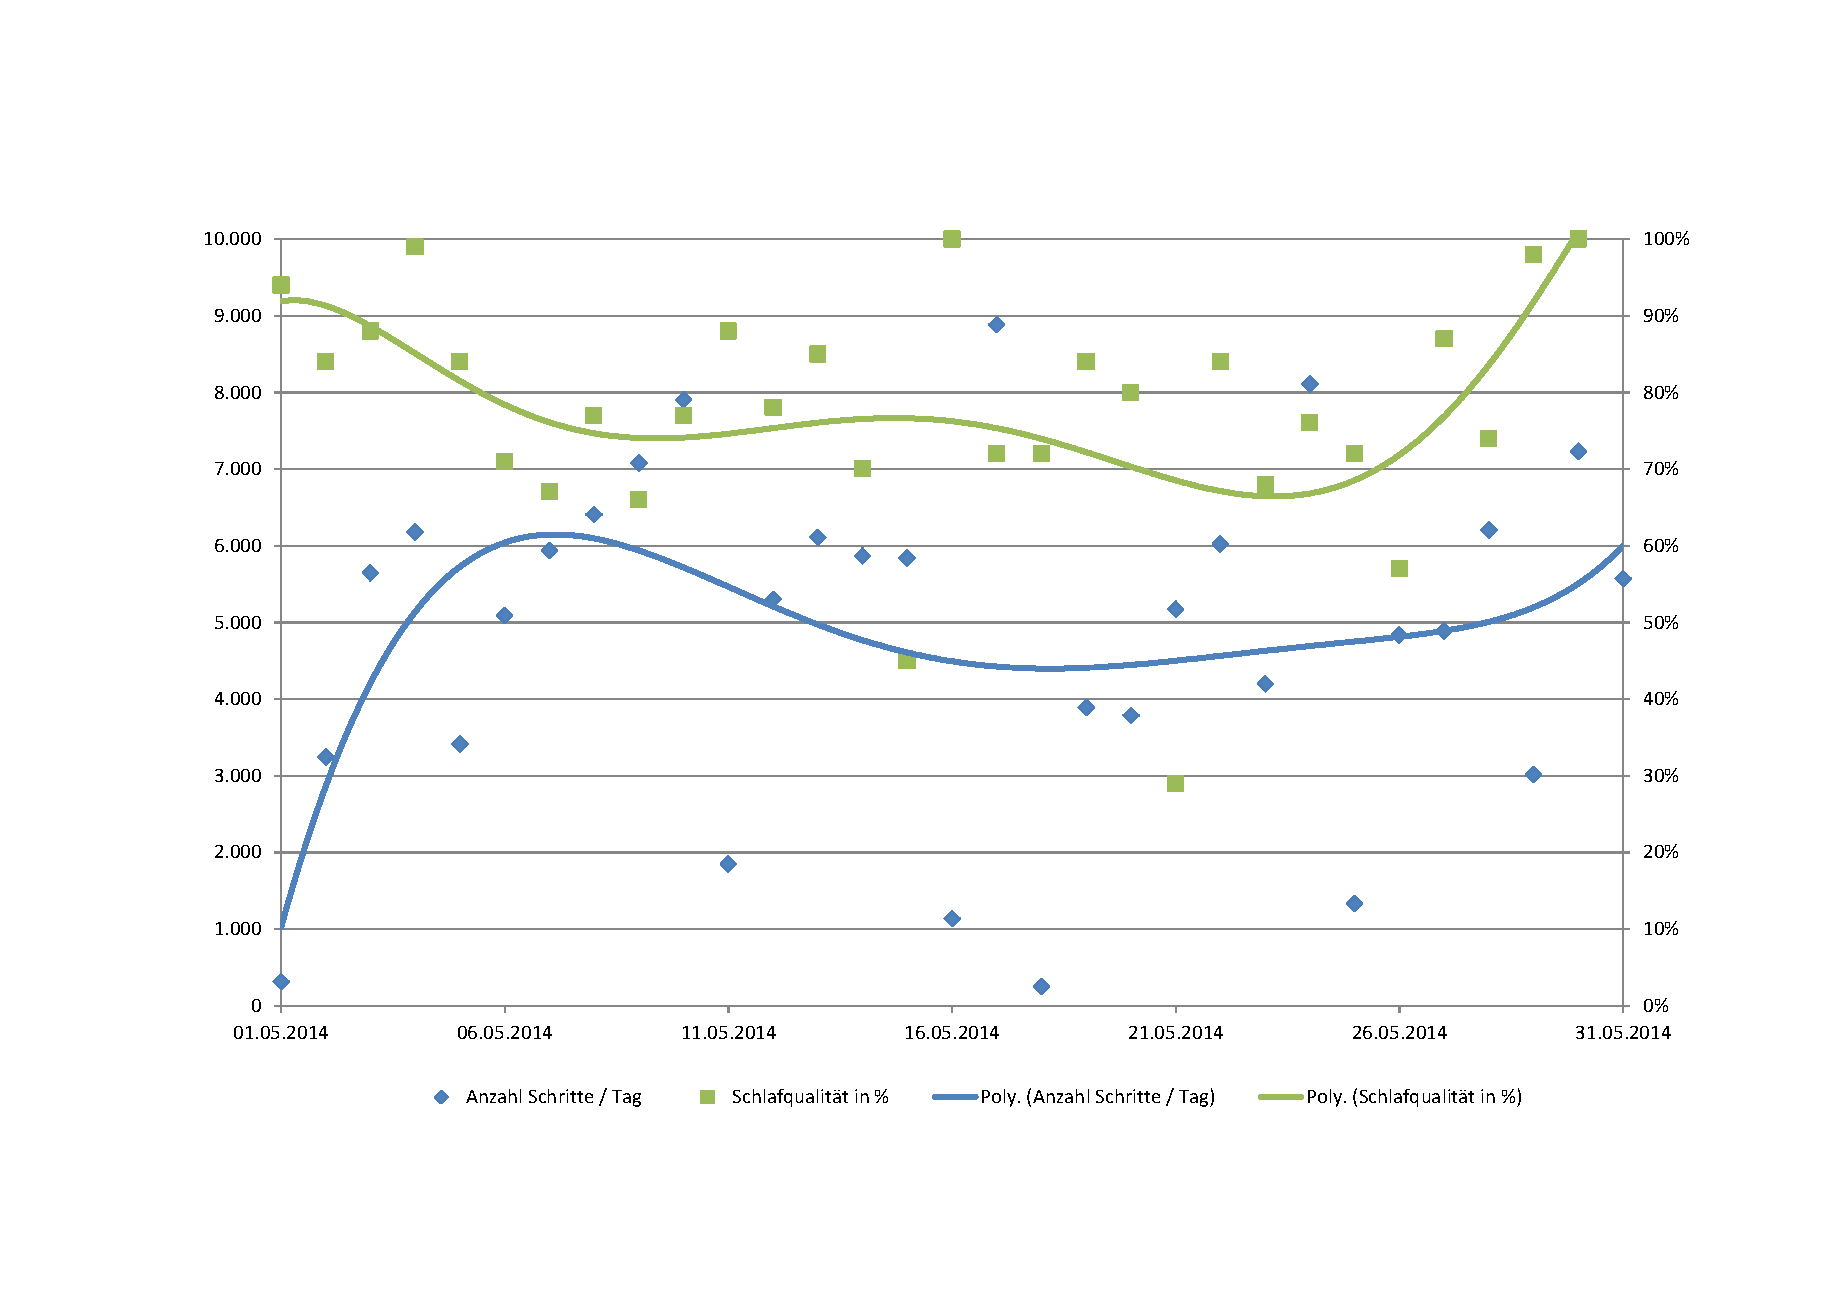
\includegraphics[angle=270,width=0.9\textwidth]{images/Analyse/Sleep-Steps} 
        \caption[Daten der Schritte pro Tag und der Schlafqualität]{Daten der Schritte pro Tag und der Schlafqualität}
        \label{fig:ZusammenhangSchlafqualitätProSchrittenAmTag}
\end{figure}

Das Diagramm \ref{fig:ZusammenhangSchlafqualitätProSchrittenAmTag} zeigt die Anzahl der aufgenommen Schritte pro Tag und zusätzlich die Schlafqualität in Prozent des jeweiligen Tages.
Die Werte der Grafik beziehen sich auf den kompletten Aufzeichnugszeitraums. 
Dabei handelt es sich bei den grünen Punkten um die einzelnen Datenpunkte der Schlafqualität, welche in Prozent auf der rechten Abzissenachse angegeben ist.
Auf der linken Abzissenachse wiederum wird die gesamte Anzahl der Schritte gezeigt, wie es auch der Legende zu entnehmen ist.
Zur besser Trend Ersichtlichkeit sind beide Datenreihen zusätzlich in einem Polynom sechsten Grades angenähert.
Diese Werte sind über den Erhebungszeitraum dargestellt.

Die Daten stammen aus dem Monat Mai des Jahres 2014.
In der Abbildung stamme die Werte Schritte pro Tag aus der im Projekt verwendeten Applikation Moves[\ref{ch:Apps:sec:Moves}]. 
Sleep Cycle[\ref{ch:Apps:sec:SleepCycle}] liefert dabei die Daten zur Schlafqualität.
Die Werte wurden im Zuge des Projektes von den Autoren erhoben.



%% ==============================
\section{Zusammenhang von Stimmung, Schlafqualität und Energieverbrauch}
%% ==============================
\label{ch:AnalyseUndEvaluierung:sec:KorrelationVonSchlafqualitätUndSchrittenAmTag}

\begin{figure}[H]
\centering
        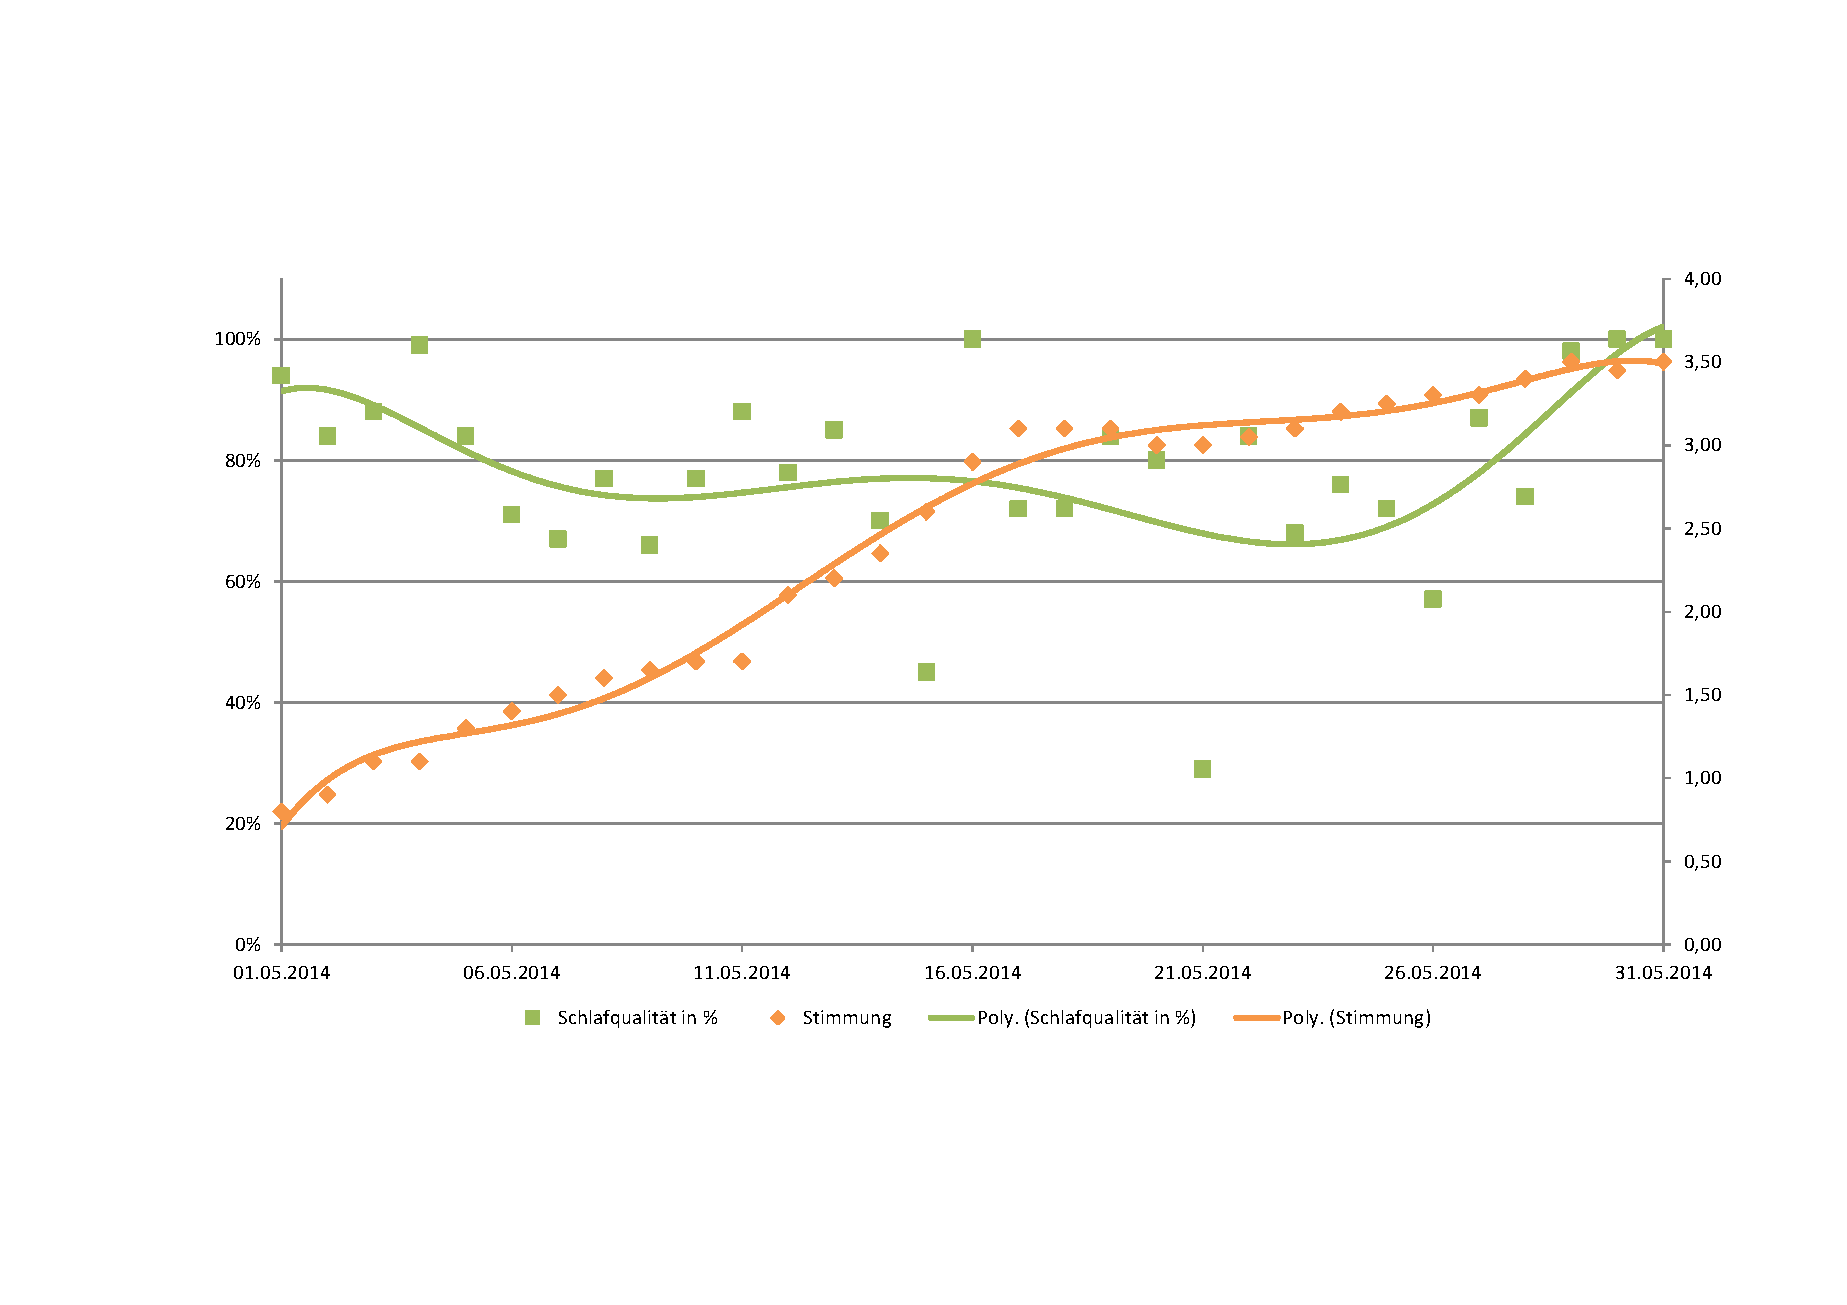
\includegraphics[angle=270,width=0.8\textwidth]{images/Analyse/Sleep-Mood} 
        \caption[Daten der Stimmung und der Schlafqualität]{Daten der Stimmung und der Schlafqualität}
        \label{fig:ZusammenhangVonStimmungUndSchlafqualität}
\end{figure}

%% ==============================
\section{Zusammenhang von Schlafqualität und Schritten am Tag}
%% ==============================
\label{ch:AnalyseUndEvaluierung:sec:KorrelationVonSchlafqualitätUndSchrittenAmTag}

\begin{figure}[H]
\centering
        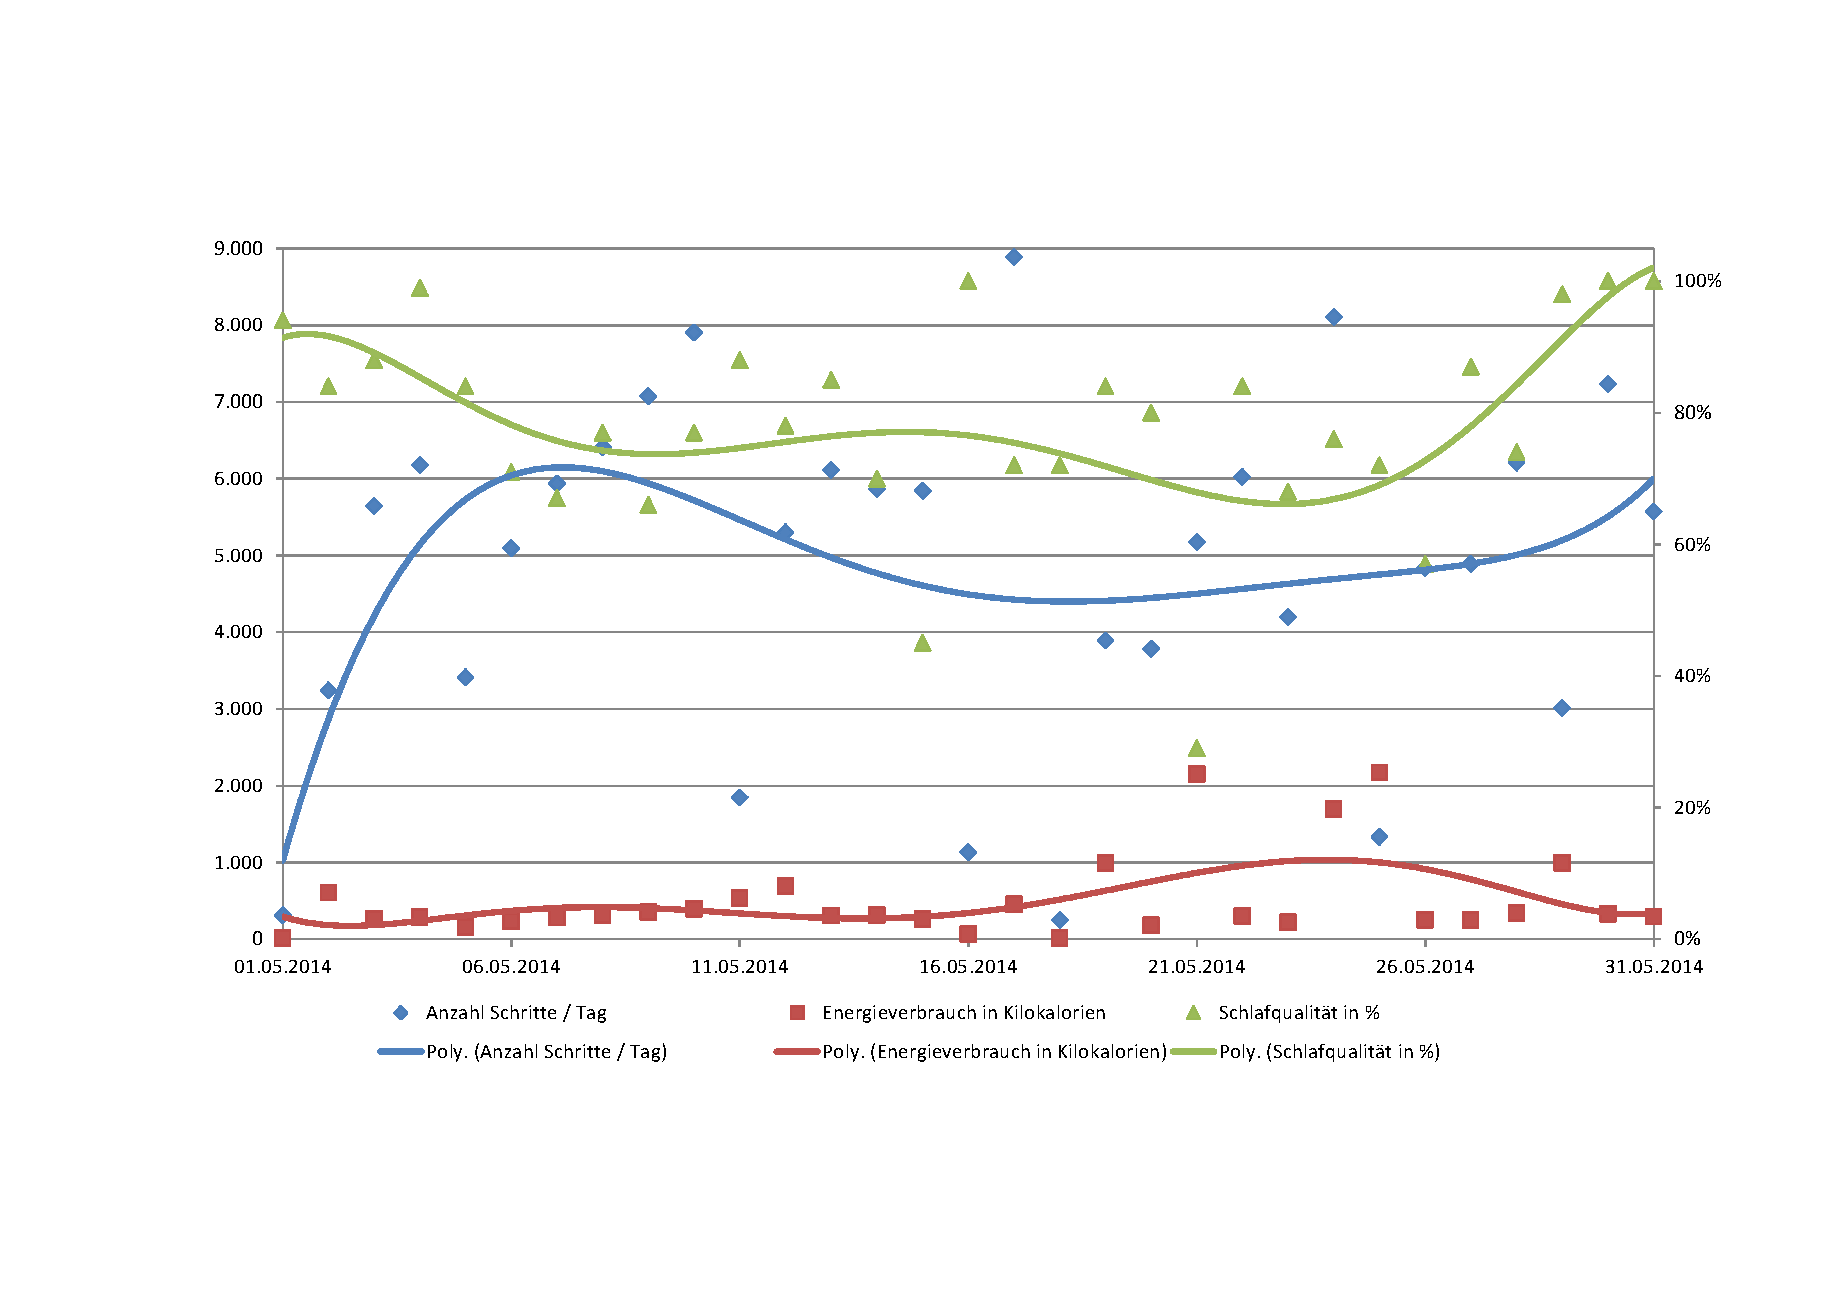
\includegraphics[angle=270,width=0.8\textwidth]{images/Analyse/Sleep-Steps-kcal} 
        \caption[Daten der Stimmung, der Schlafqualität und des Energieverbrauchs]{Daten der Stimmung, der Schlafqualität und des Energieverbrauchs}
        \label{fig:ZusammenhangVonSchlafqualitätSchrittenUndEnergieverbrauchAmTag}
\end{figure}

%% ==============================
\section{Zusammenfassung}
%% ==============================
\label{ch:Analyse:sec:zusammenfassung}


Diese Analyse liefert auf Basis einer ausführlichen Datenanalyse mit den gängigen Verfahren der Datenanalyse und -auswertung, der zuvor gewonnenen Daten, ein sehr exaktes Bild über die Zusammenhänge der jeweiligen Aktivitäten.
Die graphische Darstellung orientiert sich strikt an der Leitfrage des Projekts. 
Dadurch erhält der Leser eine erste Orientierung in welche Richtung die Beantwortung der Leitfrage ziehlen wird.

%% inferenzstatistik kann => nicht applyable weil nicht repräsentativ, referenzieren auf relativierung

%%% Local Variables: 
%%% mode: latex
%%% TeX-master: "thesis"
%%% End: 
     % Analyse
%% entwurf.tex
%% $Id: entwurf.tex 61 2012-05-03 13:58:03Z bless $
%%

\chapter{Entwurf}
\label{ch:Entwurf}
%% ==============================
In diesem Kapitel erfolgt die ausführliche Beschreibung des eigenen
Lösungsansatzes. Dabei sollten Lösungsalternativen diskutiert und
Entwurfsentscheidungen dargelegt werden.


Bla fasel\ldots

%% ==============================
\section{Abschnitt 1}
%% ==============================
\label{ch:Entwurf:sec:Abschnitt1}

Bla fasel\ldots

%% ==============================
\section{Abschnitt 2}
%% ==============================
\label{ch:Entwurf:sec:Abschnitt2}

Bla fasel\ldots

Blindtext Blindtext Blindtext Blindtext Blindtext Blindtext Blindtext
Blindtext Blindtext Blindtext Blindtext Blindtext Blindtext Blindtext
Blindtext Blindtext Blindtext Blindtext Blindtext Blindtext Blindtext
Blindtext Blindtext Blindtext Blindtext Blindtext Blindtext Blindtext
Blindtext Blindtext Blindtext Blindtext Blindtext Blindtext Blindtext
Blindtext Blindtext Blindtext Blindtext Blindtext Blindtext Blindtext
Blindtext Blindtext Blindtext Blindtext Blindtext Blindtext Blindtext
Blindtext Blindtext Blindtext Blindtext Blindtext Blindtext Blindtext
Blindtext Blindtext Blindtext Blindtext Blindtext Blindtext Blindtext
Blindtext Blindtext Blindtext Blindtext Blindtext Blindtext Blindtext
Blindtext Blindtext Blindtext Blindtext Blindtext Blindtext Blindtext
Blindtext Blindtext Blindtext Blindtext Blindtext Blindtext Blindtext
Blindtext Blindtext Blindtext Blindtext Blindtext Blindtext Blindtext
Blindtext Blindtext Blindtext Blindtext Blindtext Blindtext Blindtext
Blindtext Blindtext Blindtext Blindtext Blindtext Blindtext Blindtext
Blindtext Blindtext Blindtext Blindtext Blindtext Blindtext Blindtext
Blindtext Blindtext Blindtext Blindtext Blindtext Blindtext Blindtext

Blindtext Blindtext Blindtext Blindtext Blindtext Blindtext Blindtext
Blindtext Blindtext Blindtext Blindtext Blindtext Blindtext Blindtext
Blindtext Blindtext Blindtext Blindtext Blindtext Blindtext Blindtext
Blindtext Blindtext Blindtext Blindtext Blindtext Blindtext Blindtext
Blindtext Blindtext Blindtext Blindtext Blindtext Blindtext Blindtext
Blindtext Blindtext Blindtext Blindtext Blindtext Blindtext Blindtext
Blindtext Blindtext Blindtext Blindtext Blindtext Blindtext Blindtext
Blindtext Blindtext Blindtext Blindtext Blindtext Blindtext Blindtext
Blindtext Blindtext Blindtext Blindtext Blindtext Blindtext Blindtext
Blindtext Blindtext Blindtext Blindtext Blindtext Blindtext Blindtext
Blindtext Blindtext Blindtext Blindtext Blindtext Blindtext Blindtext
Blindtext Blindtext Blindtext Blindtext Blindtext Blindtext Blindtext
Blindtext Blindtext Blindtext Blindtext Blindtext Blindtext Blindtext
Blindtext Blindtext Blindtext Blindtext Blindtext Blindtext Blindtext
Blindtext Blindtext Blindtext Blindtext Blindtext Blindtext Blindtext
Blindtext Blindtext Blindtext Blindtext Blindtext Blindtext Blindtext
Blindtext Blindtext Blindtext Blindtext Blindtext Blindtext Blindtext
Blindtext Blindtext Blindtext Blindtext Blindtext Blindtext Blindtext
Blindtext Blindtext Blindtext Blindtext Blindtext Blindtext Blindtext
Blindtext Blindtext Blindtext Blindtext Blindtext Blindtext Blindtext

Blindtext Blindtext Blindtext Blindtext Blindtext Blindtext Blindtext
Blindtext Blindtext Blindtext Blindtext Blindtext Blindtext Blindtext
Blindtext Blindtext Blindtext Blindtext Blindtext Blindtext Blindtext
Blindtext Blindtext Blindtext Blindtext Blindtext Blindtext Blindtext
Blindtext Blindtext Blindtext Blindtext Blindtext Blindtext Blindtext
Blindtext Blindtext Blindtext Blindtext Blindtext Blindtext Blindtext
Blindtext Blindtext Blindtext Blindtext Blindtext Blindtext Blindtext
Blindtext Blindtext Blindtext Blindtext Blindtext Blindtext Blindtext
Blindtext Blindtext Blindtext Blindtext Blindtext Blindtext Blindtext
Blindtext Blindtext Blindtext Blindtext Blindtext Blindtext Blindtext
Blindtext Blindtext Blindtext Blindtext Blindtext Blindtext Blindtext
Blindtext Blindtext Blindtext Blindtext Blindtext Blindtext Blindtext
Blindtext Blindtext Blindtext Blindtext Blindtext Blindtext Blindtext
Blindtext Blindtext Blindtext Blindtext Blindtext Blindtext Blindtext
Blindtext Blindtext Blindtext Blindtext Blindtext Blindtext Blindtext

Blindtext Blindtext Blindtext Blindtext Blindtext Blindtext Blindtext
Blindtext Blindtext Blindtext Blindtext Blindtext Blindtext Blindtext
Blindtext Blindtext Blindtext Blindtext Blindtext Blindtext Blindtext
Blindtext Blindtext Blindtext Blindtext Blindtext Blindtext Blindtext
Blindtext Blindtext Blindtext Blindtext Blindtext Blindtext Blindtext
Blindtext Blindtext Blindtext Blindtext Blindtext Blindtext Blindtext
Blindtext Blindtext Blindtext Blindtext Blindtext Blindtext Blindtext
Blindtext Blindtext Blindtext Blindtext Blindtext Blindtext Blindtext
Blindtext Blindtext Blindtext Blindtext Blindtext Blindtext Blindtext
Blindtext Blindtext Blindtext Blindtext Blindtext Blindtext Blindtext
Blindtext Blindtext Blindtext Blindtext Blindtext Blindtext Blindtext
Blindtext Blindtext Blindtext Blindtext Blindtext Blindtext Blindtext
Blindtext Blindtext Blindtext Blindtext Blindtext Blindtext Blindtext
Blindtext Blindtext Blindtext Blindtext Blindtext Blindtext Blindtext
Blindtext Blindtext Blindtext Blindtext Blindtext Blindtext Blindtext
Blindtext Blindtext Blindtext Blindtext Blindtext Blindtext Blindtext

Blindtext Blindtext Blindtext Blindtext Blindtext Blindtext Blindtext
Blindtext Blindtext Blindtext Blindtext Blindtext Blindtext Blindtext
Blindtext Blindtext Blindtext Blindtext Blindtext Blindtext Blindtext
Blindtext Blindtext Blindtext Blindtext Blindtext Blindtext Blindtext
Blindtext Blindtext Blindtext Blindtext Blindtext Blindtext Blindtext
Blindtext Blindtext Blindtext Blindtext Blindtext Blindtext Blindtext
Blindtext Blindtext Blindtext Blindtext Blindtext Blindtext Blindtext
Blindtext Blindtext Blindtext Blindtext Blindtext Blindtext Blindtext
Blindtext Blindtext Blindtext Blindtext Blindtext Blindtext Blindtext
Blindtext Blindtext Blindtext Blindtext Blindtext Blindtext Blindtext
Blindtext Blindtext Blindtext Blindtext Blindtext Blindtext Blindtext
Blindtext Blindtext Blindtext Blindtext Blindtext Blindtext Blindtext
Blindtext Blindtext Blindtext Blindtext Blindtext Blindtext Blindtext

%% ==============================
\section{Zusammenfassung}
%% ==============================
\label{ch:Entwurf:sec:zusammenfassung}

Am Ende sollten ggf. die wichtigsten Ergebnisse nochmal in \emph{einem}
kurzen Absatz zusammengefasst werden.

%%% Local Variables: 
%%% mode: latex
%%% TeX-master: "thesis"
%%% End: 
     % Entwurf
%% implemen.tex
%% $Id: implemen.tex 61 2012-05-03 13:58:03Z bless $
%%

\chapter{Implementierung}
\label{ch:Implementierung}
%% ==============================
Bla fasel\ldots

%% ==============================
\section{Abschnitt 1}
%% ==============================
\label{ch:Implementierung:sec:Abschnitt1}

Bla fasel\ldots

%% ==============================
\section{Abschnitt 2}
%% ==============================
\label{ch:Implementierung:sec:Abschnitt2}

Bla fasel\ldots

%%% Local Variables: 
%%% mode: latex
%%% TeX-master: "thesis"
%%% End: 
    % Implementierung
%% eval.tex
%% $Id: eval.tex 61 2012-05-03 13:58:03Z bless $

\chapter{Evaluierung}
\label{ch:Evaluierung}
%% ==============================
Hier kommt der Nachweis, dass das in Kapitel~\ref{ch:Entwurf}
entworfene Konzept auch funktioniert. Leistungsmessungen einer
Implementierung werden auch immer gerne gesehen.

Bla fasel\ldots

%% ==============================
\section{Abschnitt 1}
%% ==============================
\label{ch:Evaluierung:sec:Abschnitt1}

Bla fasel\ldots

%% ==============================
\section{Abschnitt 2}
%% ==============================
\label{ch:Evaluierung:sec:Abschnitt2}

Bla fasel\ldots

%% ==============================
\section{Zusammenfassung}
%% ==============================
\label{ch:Evaluierung:sec:zusammenfassung}

Am Ende sollten ggf. die wichtigsten Ergebnisse nochmal in \emph{einem}
kurzen Absatz zusammengefasst werden.

%%% Local Variables: 
%%% mode: latex
%%% TeX-master: "thesis"
%%% End: 
        % Evaluierung
%% zusammenf.tex
%% $Id: zusammenf.tex 61 2012-05-03 13:58:03Z bless $
%%
% !TEX root = thesis.tex

\chapter{Zusammenfassung und Ausblick}
\label{ch:Zusammenfassung}
%% ==============================

Diese Analyse liefert auf Basis einer ausführlichen Datenanalyse mit den gängigen Verfahren der Datenanalyse und -auswertung, der zuvor gewonnenen Daten, ein sehr exaktes Bild über die Zusammenhänge der jeweiligen Aktivitäten.
Die graphische Darstellung orientiert sich strikt an der Leitfrage des Projekts. 
Dadurch erhält der Leser eine erste Orientierung in welche Richtung die Beantwortung der Leitfrage ziehlen wird.

Fazit:
Ob sich das Wohlbefinden durch Quantified Self verbessern lässt, kann man nicht durch Zahlen belegen. Es hängt von einem Selbst ab, inwiefern man sich damit besser fühlt.
*anregung motivation, interne konkurrenz(mehr laufen im projekt), ob es wirklich dazu beiträgt dass man gesünder ist ist eine andere frage, aber gefühlt fühlt man sich besser.
ziel von QS ist es nicht das leben zu verbessern, sonder dass man sich selbst besser fühlt. in sofern lässt sich die frage ob sich das wohlbefinden durch QS verbesern lässt mich ja beantworten.

%%% Local Variables: 
%%% mode: latex
%%% TeX-master: "thesis"
%%% End: 
   % Zusammenfassung und Ausblick

%% ++++++++++++++++++++++++++++++++++++++++++
%% Anhang
%% ++++++++++++++++++++++++++++++++++++++++++

\appendix
%\include{anhang_a}
%\include{anhang_b}

%% ++++++++++++++++++++++++++++++++++++++++++
%% Literatur
%% ++++++++++++++++++++++++++++++++++++++++++
%  mit dem Befehl \nocite werden auch nicht 
%  zitierte Referenzen abgedruckt
\cleardoublepage
\phantomsection
\addcontentsline{toc}{chapter}{\bibname}
%%
\nocite{*} % nur angeben, wenn auch nicht im Text zitierte Quellen 
           % erscheinen sollen
\bibliographystyle{itmabbrv} % mit abgek�rzten Vornamen der Autoren
%\bibliographystyle{gerplain} % abbrvnat unsrtnat
% spezielle Zitierstile: Labels mit vier Buchstaben und Jahreszahl
%\bibliographystyle{itmalpha}  % ausgeschriebene Vornamen der Autoren
\bibliography{thesis}
%% ++++++++++++++++++++++++++++++++++++++++++
%% Index
%% ++++++++++++++++++++++++++++++++++++++++++
\ifnotdraft{
\cleardoublepage
\phantomsection
\printindex            % Index, Stichwortverzeichnis
}
\end{document}
%% end of file
